%%%%%%%%%%%%%%%%%%%%%%%%%%%%%%%%%%%%%%%%%
% Focus Beamer Presentation
% LaTeX Template
% Version 1.0 (8/8/18)
%
% This template has been downloaded from:
% http://www.LaTeXTemplates.com
%
% Original author:
% Pasquale Africa (https://github.com/elauksap/focus-beamertheme) with modifications by 
% Vel (vel@LaTeXTemplates.com)
%
% Template license:
% GNU GPL v3.0 License
%
% Important note:
% The bibliography/references need to be compiled with bibtex.
%
%%%%%%%%%%%%%%%%%%%%%%%%%%%%%%%%%%%%%%%%%

%----------------------------------------------------------------------------------------
%	PACKAGES AND OTHER DOCUMENT CONFIGURATIONS
%----------------------------------------------------------------------------------------

\documentclass{beamer}
\usepackage[style=authoryear]{biblatex}
\usepackage{perpage}
\MakePerPage{footnote}
\addbibresource{example.bib}

\usetheme{focus} % Use the Focus theme supplied with the template
% Add option [numbering=none] to disable the footer progress bar
% Add option [numbering=fullbar] to show the footer progress bar as always full with a slide count

% Uncomment to enable the ice-blue theme
%\definecolor{main}{RGB}{92, 138, 168}
%\definecolor{background}{RGB}{240, 247, 255}

\newcommand{\vuwlogo}{%
    \begin{tikzpicture}[remember picture,overlay]
        \node[anchor=north east,yshift=3.5pt,xshift=0pt] at (current page.north east) {
\includegraphics[height=1cm]{Images/vuw.png}};
        \node[anchor=north east,yshift=3.5pt,xshift=-70pt] at (current page.north east) {
\includegraphics[height=1cm]{Images/ECRG.png}};
    \end{tikzpicture}%
}

%------------------------------------------------

\usepackage{booktabs} % Required for better table rules

%----------------------------------------------------------------------------------------
%	 TITLE SLIDE
%----------------------------------------------------------------------------------------

\title{EuroGP 2023 Recap}

\subtitle{Hot Trends in Genetic Programming}

\author{Hengzhe Zhang}

\institute{Victoria University of Wellington}

\date{26/04/2023}

%------------------------------------------------

\begin{document}

%------------------------------------------------

\begin{frame}
	\maketitle % Automatically created using the information in the commands above
	\vuwlogo
\end{frame}


\begin{frame}{Hot Trends}
\vuwlogo

According to the EuroGP 2023 article list, the hot trends in GP mainly involve:

\begin{itemize}
	\item Adaptive Methods for GP
	\item GP for Symbolic Regression
	\item Knowledge Guided GP
	\item GP for Machine Learning
	\item GP in Domain Applications
\end{itemize}
\end{frame}

\begin{frame}{Table of Contents}
	\tableofcontents
	\vuwlogo
\end{frame}

%----------------------------------------------------------------------------------------
%	 SECTION 1
%----------------------------------------------------------------------------------------
\section{Adaptive Methods for GP}
\begin{frame}{Adaptive Methods for GP}\vuwlogo
	\begin{enumerate}
		\item \fullcite{lima2023adaptive}
		\item \fullcite{ferreira2023self}
		\item \fullcite{carvalho2023context}
	\end{enumerate}
\end{frame}

\begin{frame}{Adaptive Batch Size}\vuwlogo
Adaptive Batch Size CGP: Improving Accuracy and Runtime for CGP Logic Optimization Flow~\footfullcite{lima2023adaptive}
\begin{itemize}
	\item Initialization: Start with an initial batch size ($\beta$) for evaluating individuals in the CGP population.
	\item Stagnation detection: Track the Simple Moving Average (SMA) of the accuracy over a window of $\sigma$ generations, and compare it with the previous SMA to detect stagnation.
\end{itemize}
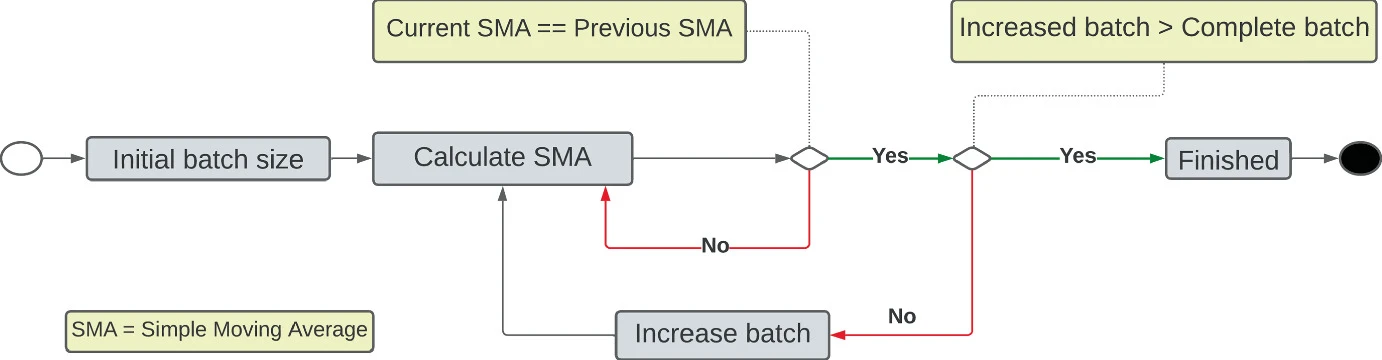
\includegraphics[width=\linewidth]{Images/AdaptiveBatch.png}
\end{frame}

\begin{frame}{Adaptive Batch Size}\vuwlogo
Adaptive Batch Size CGP: Improving Accuracy and Runtime for CGP Logic Optimization Flow~\footfullcite{lima2023adaptive}
\begin{itemize}
\item Batch size adjustment: Increase the batch size by $\alpha$ terms if stagnation is detected, provided it doesn't surpass the total available data.
\item Maximum data utilization: If all available data is being used, continue the search using the standard CGP algorithm without further ABS adjustments.
\end{itemize}
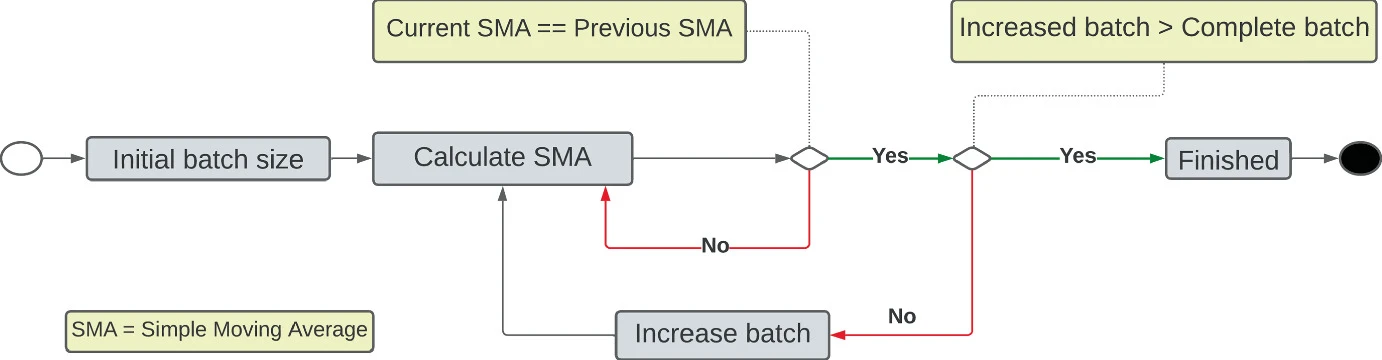
\includegraphics[width=\linewidth]{Images/AdaptiveBatch.png}
\end{frame}

\begin{frame}{Adaptive Batch Size}
	\begin{figure}
	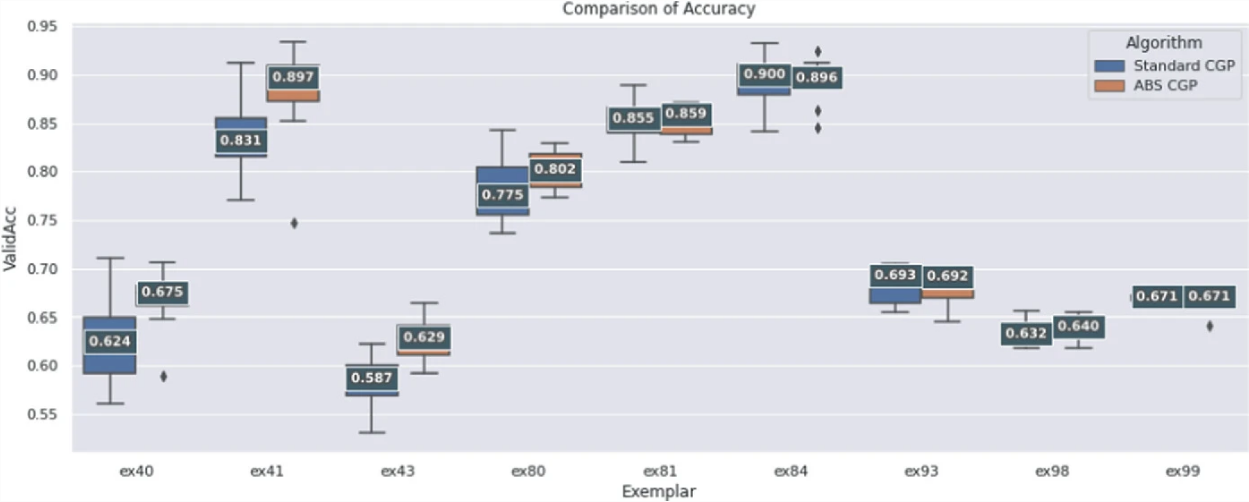
\includegraphics[width=\linewidth]{Images/AdaptiveBatchAccuracy.png}
	\caption{Accuracy of Standard CGP and ABS CGP}
	\end{figure}
\end{frame}

\begin{frame}{Adaptive Batch Size}\vuwlogo
	\begin{figure}
	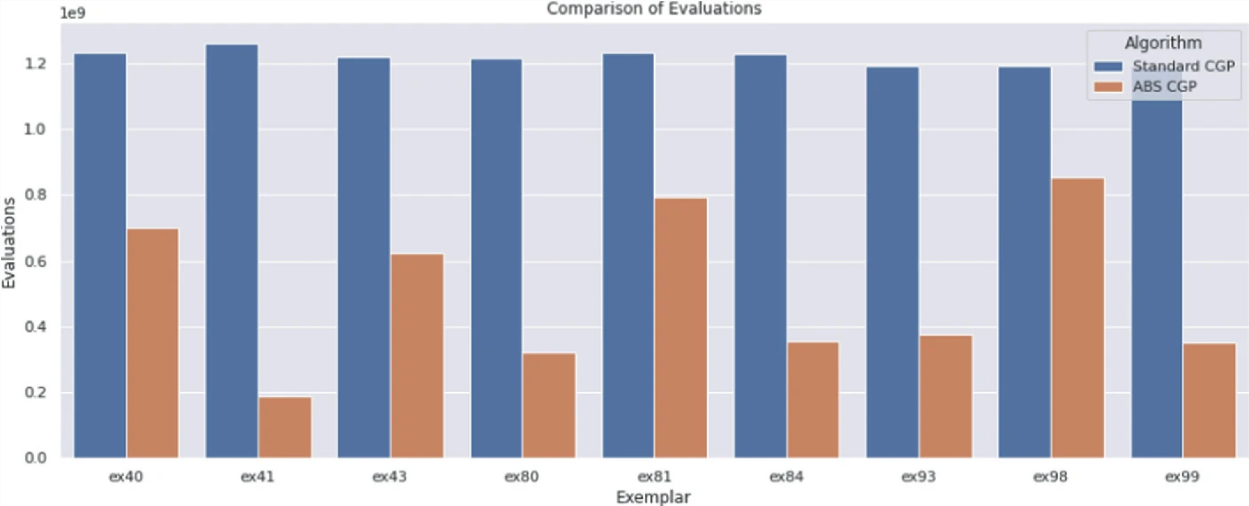
\includegraphics[width=\linewidth]{Images/AdaptiveBatchEvaluation.png}
	\caption{Number of evaluations between ABS CGP and Standard CGP}
	\end{figure}
\end{frame}

\begin{frame}{Adaptive Mutation for GP}\vuwlogo
Context Matters: Adaptive Mutation for Grammars~\footfullcite{carvalho2023context}
\begin{enumerate}
\item Initialize a population of individuals, each carrying a mutation array containing mutation probabilities for each non-terminal.
\item Determine which non-terminals to mutate based on the mutation probabilities.
\end{enumerate}
\begin{center}
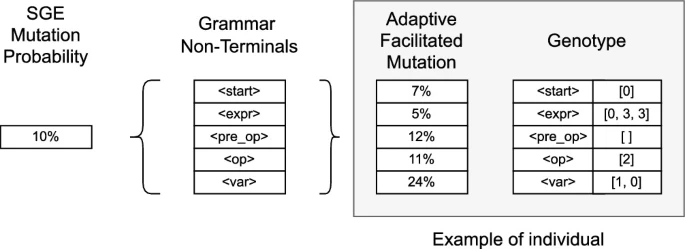
\includegraphics[width=0.8\linewidth]{Images/AdaptiveMutation.png}
\end{center}
\end{frame}

\begin{frame}{Adaptive Mutation for GP}\vuwlogo
Context Matters: Adaptive Mutation for Grammars~\footfullcite{carvalho2023context}
\begin{enumerate}
\item During each generation, adjust the mutation probabilities in the mutation array using a random value sampled from a Gaussian distribution with mean 0 and a configurable standard deviation ($\sigma$).
\item During crossover, offspring inherit the mutation array from their fittest parent.
\end{enumerate}
\begin{center}
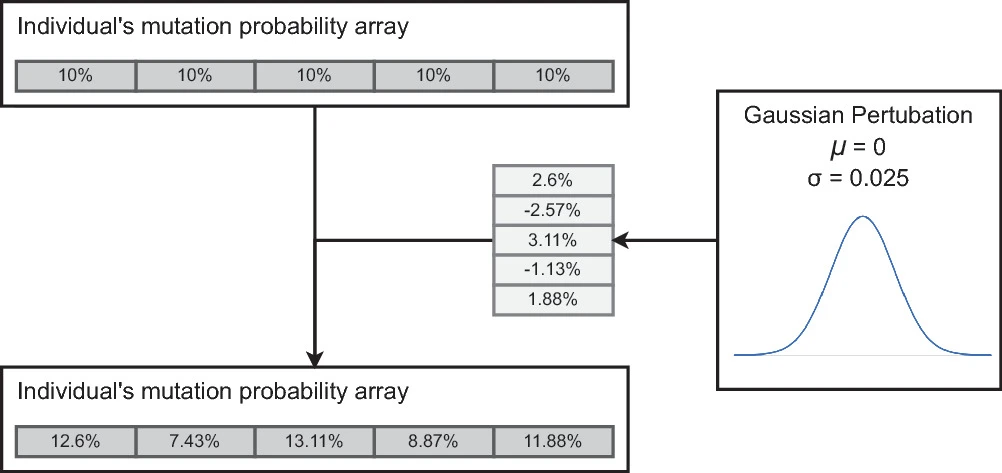
\includegraphics[width=0.65\linewidth]{Images/ProbabilityMutation.png}
\end{center}
\end{frame}

\begin{frame}{Adaptive Mutation for GP}\vuwlogo
\begin{center}
	\begin{figure}
		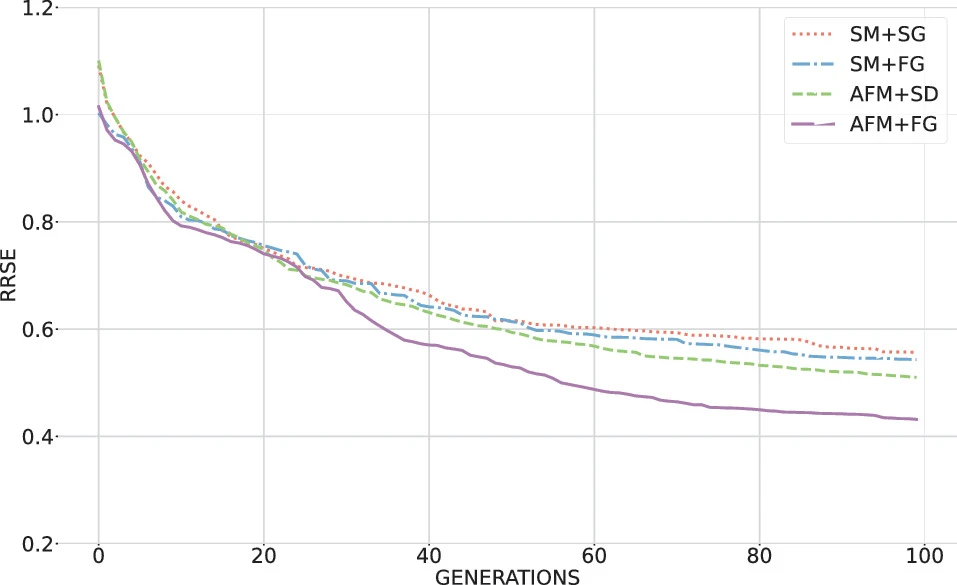
\includegraphics[width=0.8\linewidth]{Images/Pagie.png}
		\caption{The mean best fitness of 100 runs for the Pagie polynomial.}
	\end{figure}
\end{center}
\end{frame}

\begin{frame}{Adaptive Mutation for GP}\vuwlogo
\begin{center}
	\begin{figure}
		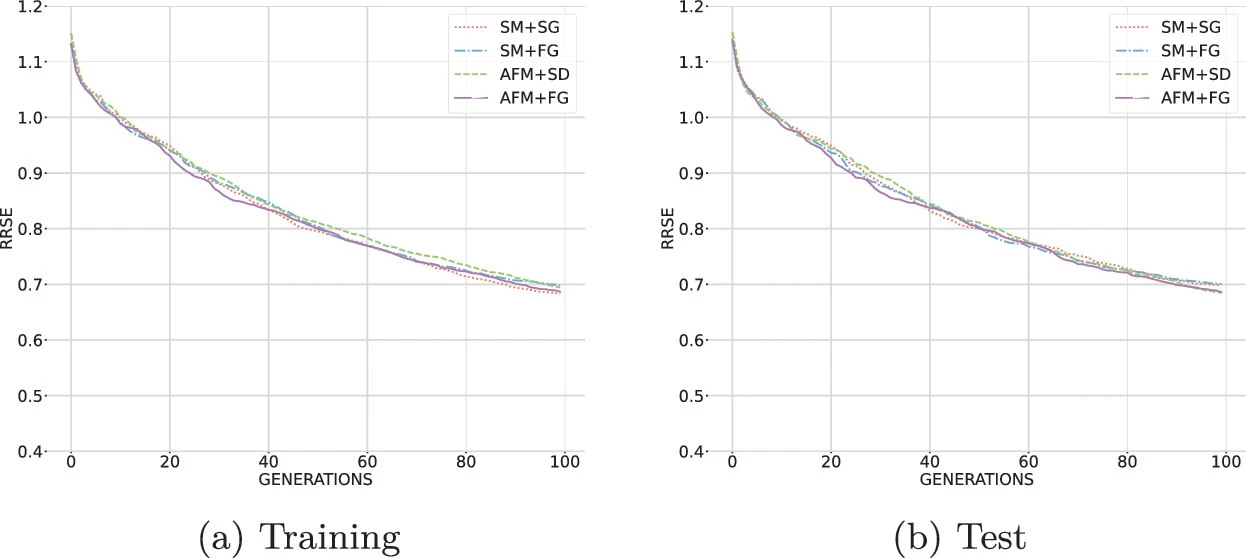
\includegraphics[width=\linewidth]{Images/BostonHousing.png}
		\caption{The mean best fitness of 100 runs for the Boston Housing dataset.}
	\end{figure}
\end{center}
\end{frame}

\section{Genetic Programming for SR}
\begin{frame}{Genetic Programming for SR}\vuwlogo
	\begin{enumerate}
		\item \fullcite{wittenberg2023small}
		\item \fullcite{hu2023phenotype}
		\item \fullcite{leite2023memetic}
	\end{enumerate}
\end{frame}

\begin{frame}{DAE-GP}\vuwlogo
Small Solutions for Real-World Symbolic Regression Using Denoising Autoencoder Genetic Programming~\footfullcite{wittenberg2023small}\\
\textbf{Step 1: Model Building}
\begin{enumerate}
\item Select promising candidate solutions to form a training set $X$
\item Split training set into training and validation sets
\item Apply Levenshtein tree edit denoising strategy with chosen corruption strength (edit percentage p)
\item Train DAE-LSTM on denoised solutions to reconstruct original (uncorrupted) solutions
\item Calculate reconstruction error and update model parameters using gradient descent
\item Apply early stopping based on the validation set
\end{enumerate}
\end{frame}

\begin{frame}{DAE-GP}\vuwlogo
\textbf{Step 2: Model Sampling}~\footfullcite{zhan2022learning}
\begin{enumerate}
\item Select random candidate solutions from the training set
\item Apply the same denoising strategy as during model building
\item Propagate denoised solutions through the trained DAE-LSTM to generate new offspring candidate solutions
\item Ensure generated offspring solutions are syntactically valid
\end{enumerate}

\textbf{Step 3: Evaluate and Update}
\begin{enumerate}
\item Evaluate fitness of offspring population using the problem-specific fitness function
\item Update parent population by selecting the best individuals from parent and offspring populations
\end{enumerate}
\end{frame}

\begin{frame}{DAE-GP}\vuwlogo
	\begin{figure}
		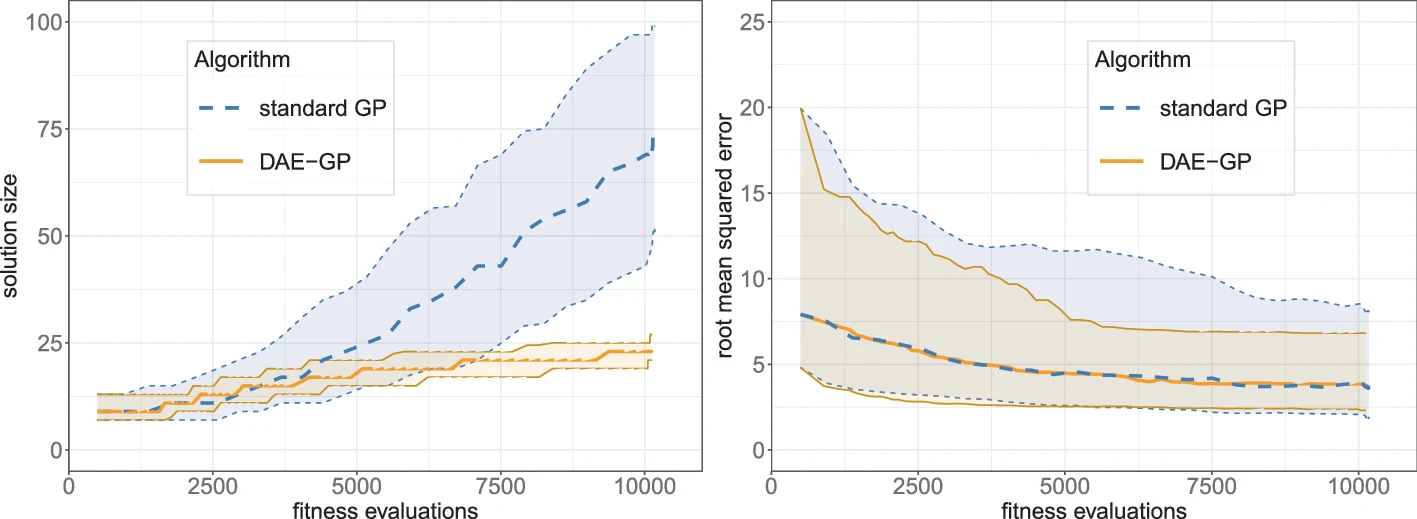
\includegraphics[width=\linewidth]{Images/DAEGPSolutionSize.png}
		\caption{Median solution size (left) and median fitness on test set (right) of best candidate solution over fitness evaluations across all datasets.}
	\end{figure}
\end{frame}

\begin{frame}{DAE-GP}\vuwlogo
	\begin{figure}
		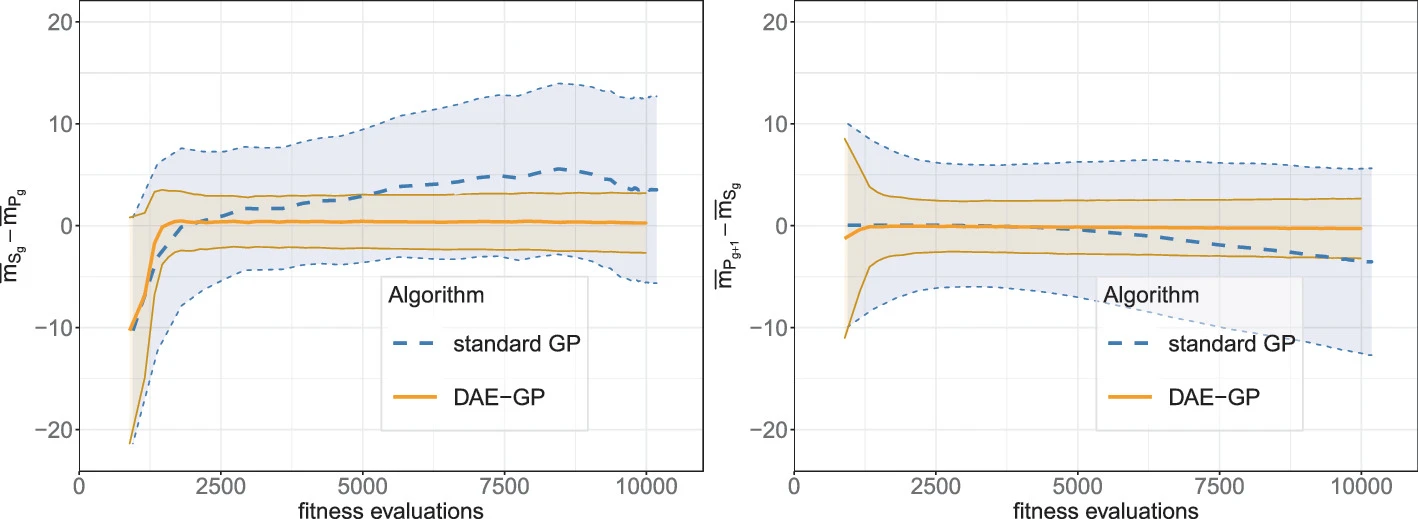
\includegraphics[width=\linewidth]{Images/SelectionBias.png}
		\caption{Bias of selection step (left) and variation step (right) on solution size measured by average differences in solution size $m$ between populations $P$ over fitness evaluations across all datasets.}
	\end{figure}
\end{frame}

\section{Knowledge Guided GP}
\begin{frame}{Knowledge Guided GP}\vuwlogo
	\begin{enumerate}
		\item \fullcite{reuter2023graph}
		\item \fullcite{kowalczykiewicz2023grammatical}
	\end{enumerate}
\end{frame}
\begin{frame}{GNN Guided GP}\vuwlogo
	Graph Networks as Inductive Bias for Genetic Programming: Symbolic Models for Particle-Laden Flows~\footfullcite{reuter2023graph}
	\begin{enumerate}
	\item Choose one of the two GN structures: $y=g(x)$ (predicting the target variable by summing the edge messages) or $y=f(g(x))$ (predicting the target variable by applying a function on the summed edge messages).
	\item Train a Graph Network (GN) on the input data (positions, velocities, etc. of the particles).
	\end{enumerate}
	\begin{center}
	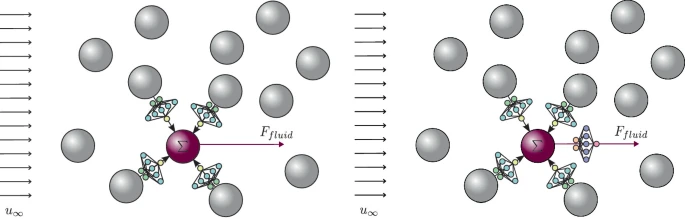
\includegraphics[width=0.65\linewidth]{Images/GNNModel.png}
	\end{center}
\end{frame}

\begin{frame}{GNN Guided GP}\vuwlogo
	Graph Networks as Inductive Bias for Genetic Programming: Symbolic Models for Particle-Laden Flows~\footfullcite{reuter2023graph}
	\begin{enumerate}
		\item Use Genetic Programming (GP) to fit symbolic models ($\Phi_e'$ and $\Phi_n'$) to the outputs of the edge and node models of the GN.
		\item Refit the constants in the symbolic models using a regression algorithm (e.g., Levenberg-Marquardt).
		\item Predict the fluid force $F_{fluid}$ using the fitted symbolic models.
	\end{enumerate}
	\begin{center}
	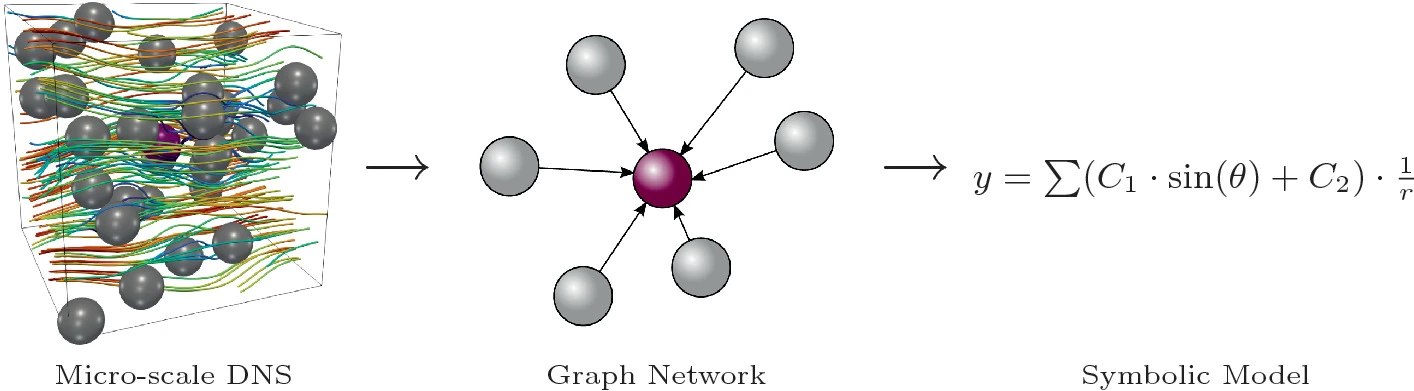
\includegraphics[width=0.65\linewidth]{Images/GNNSR.png}
	\end{center}
\end{frame}

\begin{frame}{GNN Guided GP}\vuwlogo
	\begin{figure}
		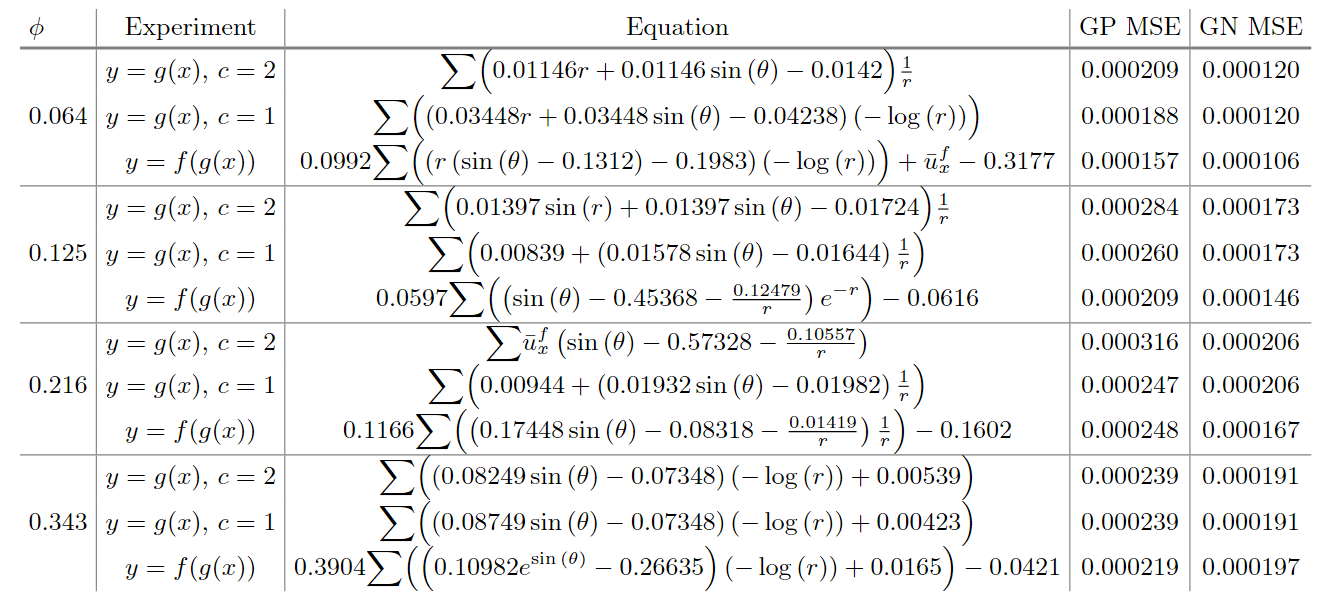
\includegraphics[width=\linewidth]{Images/GNNSRResults.png}
		\caption{Symbolic models with constants refitted to the original dataset. }
	\end{figure}
\end{frame}

\section{Genetic Programming for ML}
\begin{frame}{Genetic Programming for ML}\vuwlogo
	\begin{enumerate}
		\item \fullcite{matsumoto2023faster}
		\item \fullcite{zhou2023boosting}
		\item \fullcite{zhang2023map}
	\end{enumerate}
\end{frame}

\begin{frame}{GP for AutoML}\vuwlogo
Faster Convergence with Lexicase Selection in Tree-Based Automated Machine Learning~\footfullcite{matsumoto2023faster}
\begin{figure}
	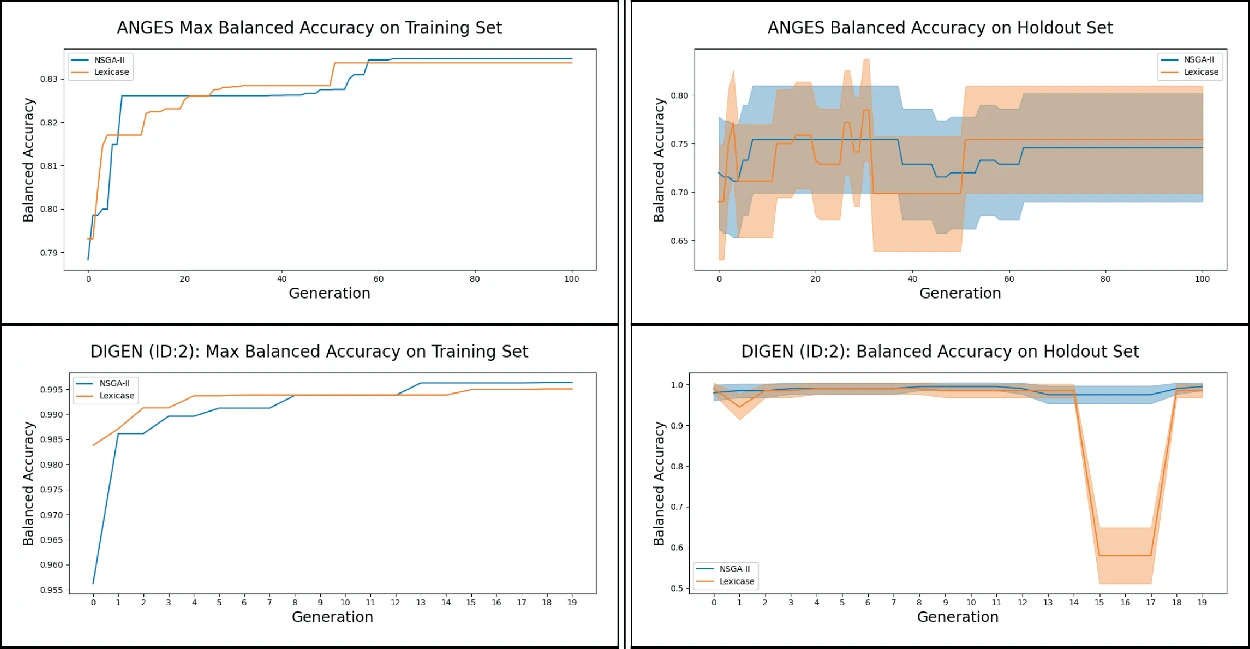
\includegraphics[width=0.65\linewidth]{Images/Lexicase.png}
	\caption{Left: Best model based on training accuracy. Right: Holdout scores for the best models based on training accuracy.}
\end{figure}
\end{frame}

\section{GP in Domain Applications}
\begin{frame}{GP in Domain Applications}\vuwlogo
	\begin{enumerate}
		\item \fullcite{miralavy2023spatial}
		\item \fullcite{djurasevic2023bias}
		\item \fullcite{de2023interacting}
	\end{enumerate}
\end{frame}

\begin{frame}{GP in DFJSS}\vuwlogo
	To Bias or Not to Bias: Probabilistic Initialisation for Evolving Dispatching Rules~\footfullcite{djurasevic2023bias}
	\begin{enumerate}
		\item The algorithm introduces a bias in selecting certain primitives at certain positions based on their frequency in the best individuals from previous experiments.
		\item Level-based probability is calculated by considering the frequency of each primitive at each level of the tree.
		\item Conditional probability takes into account the context, which consists of the parent and sibling nodes.
	\end{enumerate}
\end{frame}

\begin{frame}{GP in DFJSS}\vuwlogo
	\begin{figure}
		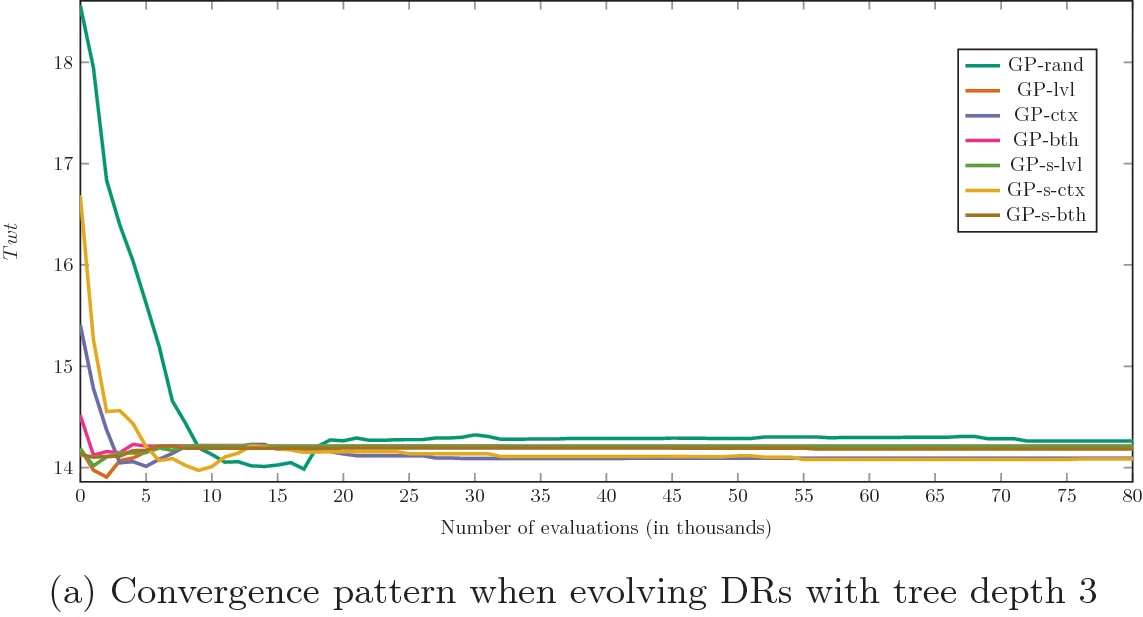
\includegraphics[width=\linewidth]{Images/Bias.png}
		\caption{Convergence patterns when evolving DRs with various initialisation methods}
	\end{figure}
\end{frame}

\begin{frame}{Conclusion}\vuwlogo
	The hot trends at EuroGP 2023 mainly involve research in:
	\begin{itemize}
		\item Developing Adaptive Methods for GP
		\item Applying Neural Networks in GP
		\item Applying GP in Machine Learning
		\item Exploring Domain Applications using GP
	\end{itemize}
	In summary, these trends focus to promote the fusion and development of genetic programming, evolutionary computation and machine learning to solve problems in practical applications.
\end{frame}

% %------------------------------------------------

\begin{frame}[focus]
	Thanks for listening!
\end{frame}

%----------------------------------------------------------------------------------------
%	 CLOSING/SUPPLEMENTARY SLIDES
%----------------------------------------------------------------------------------------

\appendix

% \begin{frame}{References}
% 	\nocite{*} % Display all references regardless of if they were cited
% 	\bibliography{example.bib}
% 	\bibliographystyle{plain}
% \end{frame}

%------------------------------------------------

% \begin{frame}{Backup Slide}
% 	This is a backup slide, useful to include additional materials to answer questions from the audience.
% 	\vfill
% 	The package \texttt{appendixnumberbeamer} is used to refrain from numbering appendix slides.
% \end{frame}

%----------------------------------------------------------------------------------------

\end{document}
